\documentclass[12pt]{article}

\usepackage{sbc-template}
\usepackage{graphicx,url}
\usepackage[utf8]{inputenc}
\usepackage[brazil]{babel}
\usepackage{amsmath, amssymb, amsthm}
%\usepackage[latin1]{inputenc}  


\sloppy

\title{Sistemas de Banco de Dados Vetoriais}

\author{Enzo Furegatti Spinellal\inst{1}, Ísis Ardisson Logullo\inst{1}, Luiz Fernando de Freitas Fernandes\inst{1},\\ Matheus Rodrigues da Silva espalaor\inst{1} }


\address{Instituto de Matemática, Estatística e Ciência da Computação - Universidade de São Paulo  (USP)\\
	\email{enzo.spinella@usp.br, isis.logullo@usp.br}
	\email{luiz.f.f.fernandes@usp.br, matheus.espalaor@usp.br}
}

\begin{document} 
	
	\maketitle
	
    \begin{abstract}
      The continuous growth of unstructured data has led to a paradigm shift in modern computing, heavily accelerated by Deep Learning and Transformer-based models. These architectures map complex semantics into high-dimensional numerical representations known as embeddings. However, traditional relational and NoSQL database management systems fail to efficiently index and query billions of dense vectors due to the curse of dimensionality. This phenomenon invalidates geometric pruning in spatial trees, forcing inefficient exhaustive linear scans. To address this infrastructure bottleneck, Vector Database Management Systems have emerged. This paper provides a structured comparative analysis of vector databases, exploring similarity metrics and Approximate Nearest Neighbor (ANN) algorithms to support real-time applications such as RAG, multimodal search, and advanced recommendation systems.
    \end{abstract}
    
    \begin{resumo} 
      O crescimento contínuo de dados não estruturados gerou uma transição de paradigma na computação moderna, impulsionada por modelos de Deep Learning e Transformers. Essas arquiteturas mapeiam a semântica de dados complexos em representações numéricas contínuas chamadas embeddings. No entanto, os SGBDs tradicionais (relacionais e NoSQL) falham ao indexar e consultar bilhões de vetores densos devido à maldição da dimensionalidade. Esse fenômeno invalida a poda geométrica em árvores espaciais, forçando varreduras lineares exaustivas e ineficientes. Para mitigar esse gargalo de infraestrutura, surgiram os Sistemas de Bancos de Dados Vetoriais. Este trabalho apresenta uma análise comparativa dessas ferramentas, explorando métricas de similaridade e algoritmos de Vizinhos Mais Próximos Aproximados (ANN) para sustentar aplicações em tempo real como RAG, busca multimodal e recomendação.
    \end{resumo}	
	
	\section{Contextualização e Motivação} \label{sec:motivacao}
	
	\subsection{O Boom dos Modelos de Linguagem de Grande Porte (LLMs) e Dados Não Estruturados}
	
	A computação moderna enfrenta uma transição de paradigma na natureza dos dados gerados globalmente. Estima-se que mais de 80\% das informações produzidas por corporações e usuários consistam em dados não estruturados, tais como textos em linguagem natural, imagens, áudios e fluxos de vídeo. Historicamente, a extração desses valores dependia de metadados textuais preenchidos manualmente ou técnicas rígidas de processamento de linguagem natural baseadas em palavras-chave.

    A ascensão dos modelos de Deep Learning, consolidados pelas arquiteturas de \textbf{Transformers}, revolucionou esse cenário. Redes neurais modernas são capazes de mapear a semântica latente de dados complexos e traduzi-los em representações numéricas contínuas conhecidas como \textbf{Embeddings} de alta dimensionalidade. Desse modo, dois blocos de texto com construções sintáticas completamente distintas são projetados em regiões geometricamente próximas dentro de um espaço vetorial, permitindo que computadores executem a \textbf{busca semântica}.

    Os \textbf{Large Language Models (LLMs)} representam o ápice dessa evolução no aprendizado de representações ponta a ponta aplicadas à linguagem natural. Estruturalmente, um LLM é um modelo autoregressivo baseado na arquitetura Transformer, composto por bilhões de parâmetros que são treinados de forma auto-supervisionada em \textit{corpora} (dados com curadoria, limpeza, filtragem de conteúdo ofensivo e formatação para processar de maneira padronizada) textuais massivos à escala da internet \cite {zhao2023survey}. 
    
    O princípio fundamental de um LLM reside na tarefa de modelagem de linguagem causal, cujo objetivo matemático é prever a probabilidade do próximo token dado um histórico de tokens anteriores. Ao otimizar essa função de perda em larga escala através do mecanismo de Self-Attention, o modelo não apenas decora regras gramaticais, mas desenvolve propriedades emergentes — capacidades cognitivas complexas e comportamentos de raciocínio que não foram explicitamente programados, surgindo puramente devido à escala de parâmetros e volume de dados. Dessa forma, os LLMs atuam como motores de inferência capazes de compreender contextos sutis, responder a instruções em linguagem natural e mapear conceitos abstratos no espaço latente de seus embeddings.

	Até meados de 2017, o processamento de dados sequenciais baseava-se em Redes Neurais Recorrentes e suas variantes. Essas redes processavam o texto de forma estritamente sequencial, token por token, o que gerava dois gargalos intransponíveis: a impossibilidade de paralelização do treinamento em larga escala e o problema do desvanecimento do gradiente, limitando a capacidade de reter dependências contextuais de longo alcance no texto.
	
	A arquitetura \textbf{Transformer}, introduzida por Vaswani \cite{vaswani2017attention} e consolidada em pesquisas recentes, rompeu essa limitação ao eliminar completamente a recorrência e basear-se exclusivamente no Mecanismo de Self-Attention. O Self-Attention permite que cada token em uma sequência olhe para todas as outras palavras simultaneamente, calculando dinamicamente um peso de relevância mútua, independentemente da distância física entre elas no texto.

    \begin{figure}[ht]
        \centering
        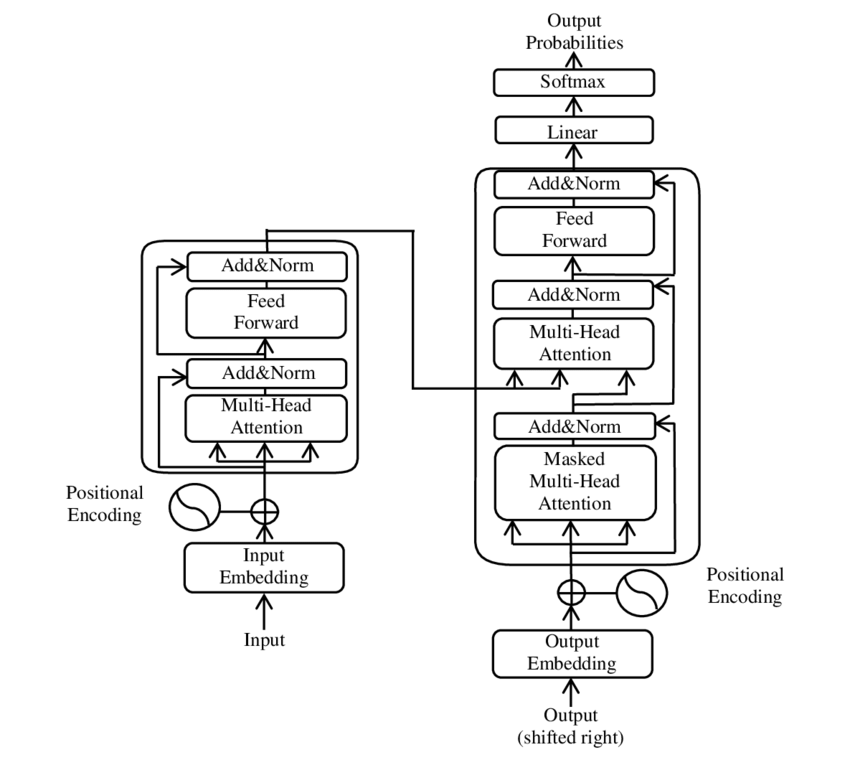
\includegraphics[width=.5\textwidth]{transformer.png}
        \caption{Estrutura Transformer}
        \label{fig:Transformer}
	\end{figure}
    
	Como as arquiteturas de computadores e os modelos matemáticos operam estritamente sobre matrizes numéricas, é necessário traduzir entidades discretas do mundo real (palavras, imagens pixeladas, áudios) em entidades contínuas. Um \textbf{Embedding} é uma representação vetorial densa de uma entidade em um espaço contínuo de alta dimensionalidade, projetada de modo que a estrutura geométrica desse espaço reflita as propriedades semânticas subjacentes do domínio original.
	
	O \textbf{Deep Learning} é um subcampo do Machine Learning fundamentado em arquiteturas de Redes Neurais Artificiais com múltiplas camadas ocultas interconectadas. Ao contrário dos algoritmos tradicionais de aprendizado supervisionado, que dependem criticamente de engenharia de atributos manual, o Deep Learning introduz o conceito de aprendizado de representação ponta a ponta.
	
	\subsection{Limitações dos SGBDs Tradicionais}
	
	Os Sistemas de Gerenciamento de Bancos de Dados (SGBDs) tradicionais, sejam relacionais (SQL) baseados na álgebra relacional ou NoSQL (documentais, chave-valor) baseados em hashing e árvores B+, foram projetados para responder a correspondências exatas, ordenação escalar e lógica booleana.
	
	Quando confrontados com a necessidade de indexar e consultar bilhões de vetores densos, os índices tradicionais falham \cite{malkov2020efficient}. A indexação em árvores multidimensionais tradicionais (como R-Trees ou $K\text{-d}$-Trees) sofre uma degradação exponencial de desempenho à medida que o número de dimensões aumenta, um fenômeno conhecido na literatura como a \textbf{maldição da dimensionalidade}. Como consequência, o SGBD é forçado a recorrer a uma busca de varredura sequencial, tornando o tempo de resposta impraticável para aplicações em tempo real.
    
    O advento dos modelos de Deep Learning introduziu a necessidade de indexar e consultar bilhões de vetores densos (como os embeddings de alta dimensionalidade). Quando confrontados com essa demanda, os índices e paradigmas tradicionais colapsam por completo.
    
    Somando-se à ineficiência algorítmica, há uma grave limitação de hardware e arquitetura de memória nos SGBDs tradicionais. Os algoritmos de cálculo de distância vetorial exigem acessos massivos e contínuos à memória RAM ou, pior, paginação de disco. Como os índices tradicionais não foram desenhados para paralelização a nível de instrução em nível de CPU/GPU (técnicas como SIMD - Single Instruction, Multiple Data), o processamento dessa varredura linear torna o tempo de resposta proibitivo para sistemas industriais que exigem subsegundos ou milissegundos para aplicações em tempo real.
	
	\subsection{Aplicações Modernas e a Infraestrutura Vetorial}
	
	Para contornar essa limitação e sustentar a nova onda de aplicações de Inteligência Artificial, surgiram os \textbf{Sistemas de Bancos de Dados Vetoriais}. Eles atuam como a infraestrutura central para o armazenamento, indexação persistente e recuperação eficiente de vetores de características. Entre as aplicações mais proeminentes, destacam-se:
	
	\begin{itemize}
		\item \textbf{Retrieval-Augmented Generation (RAG)} \cite{lewis2020retrieval}: Esta arquitetura resolve uma das principais limitações das grandes barreiras de modelos de linguagem (LLMs) - a volatilidade do conhecimento estático de seus pesos de treinamento e a propensão a alucinações. O processo opera em um fluxo bidirecional. Primeiro, no estágio de ingestão, documentos corporativos ou bases de dados textuais são fragmentados e convertidos em vetores densos para popular o banco vetorial. No momento da inferência, a consulta do usuário é submetida ao mesmo modelo de embedding, e o banco vetorial executa uma busca por similaridade de cosseno ou produto interno para extrair os fragmentos de texto semanticamente mais relevantes. Esse contexto recuperado é injetado dinamicamente no prompt enviado ao LLM. Como resultado, o modelo gera uma resposta fundamentada em evidências em tempo real, delimitada pelo contexto provido, sem a necessidade de re-treinamento ou \textit{fine-tuning} dispendiosos.

        \begin{figure}[ht]
            \centering
            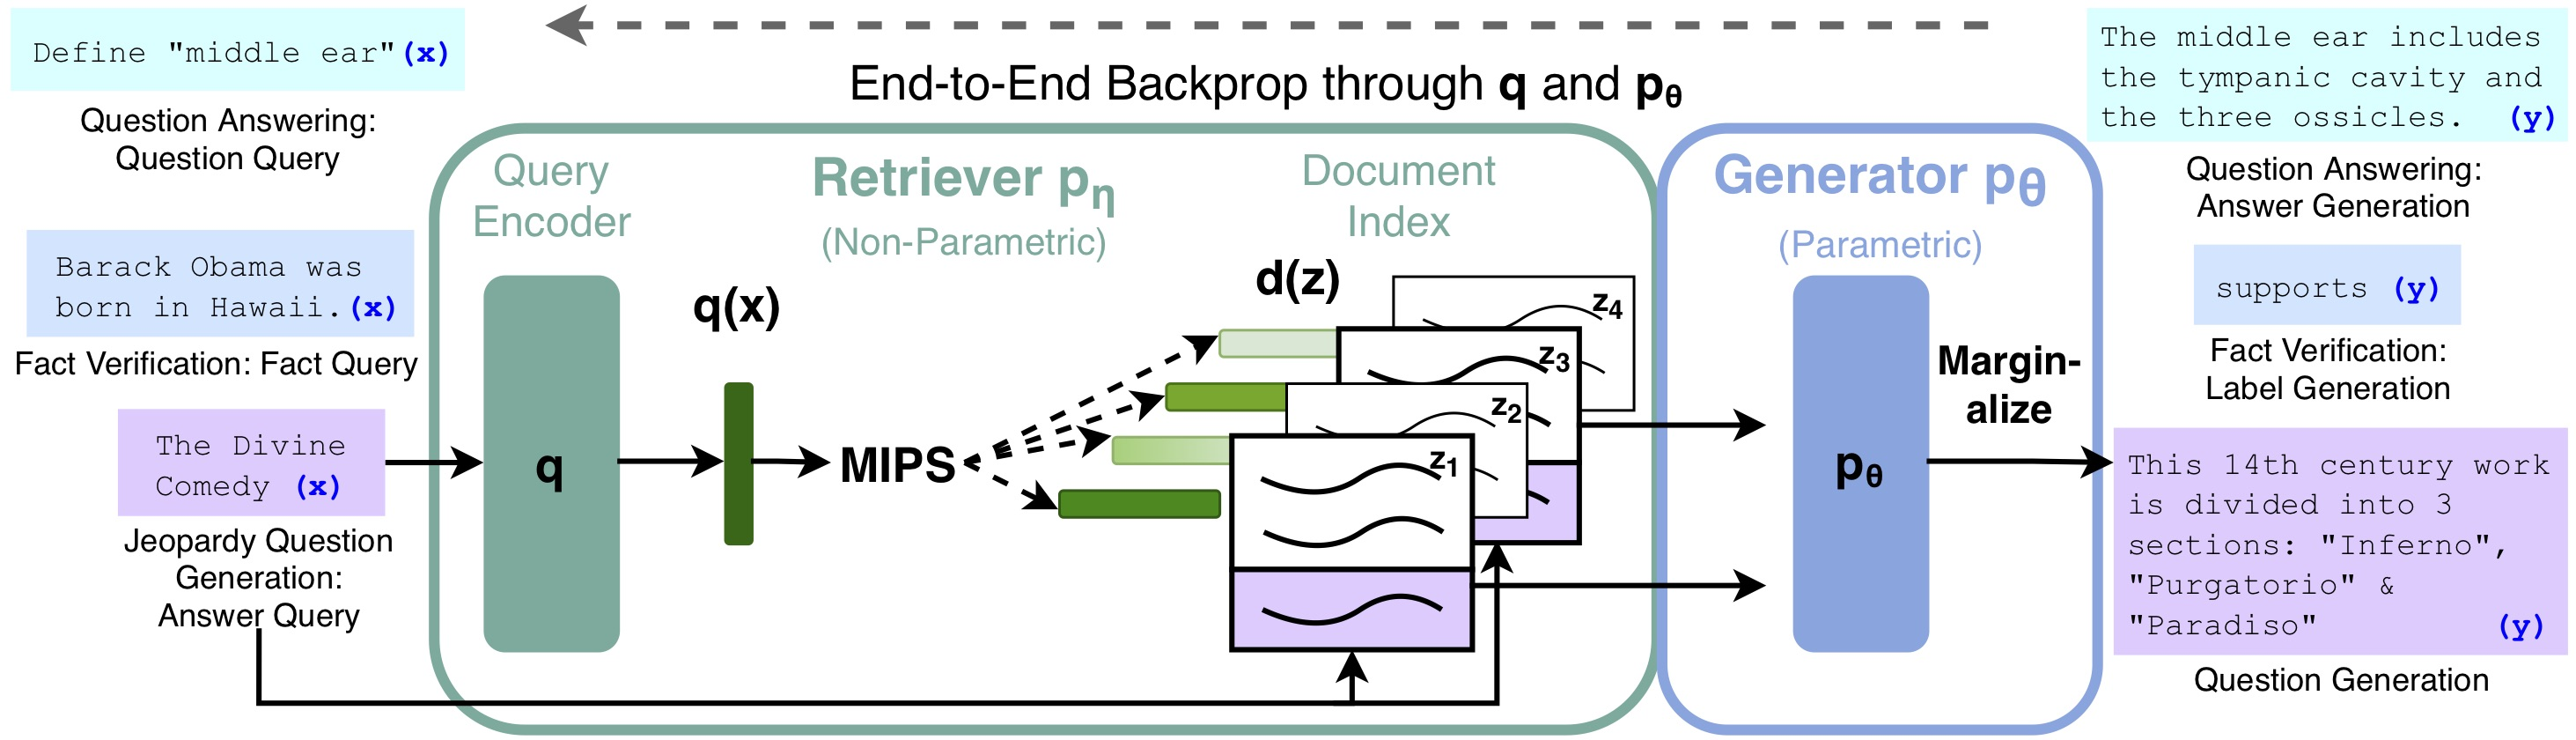
\includegraphics[width=.5\textwidth]{RAG.jpg}
            \caption{Fluxo RAG}
            \label{fig:RAG}
	    \end{figure}
        
		\item \textbf{Busca Semântica Multimodal}: Sistemas de busca tradicionais dependem estritamente de metadados textuais estruturados ou correspondências exatas de tokens. A busca multimodal rompe essa barreira ao unificar dados de diferentes naturezas — como textos, imagens, áudios e vídeos — dentro de um mesmo espaço vetorial latente compartilhado. Isso é viabilizado por codificadores bi-encoder (como a arquitetura CLIP \cite{radford2021learning}). Esses modelos são treinados para projetar conceitos equivalentes em coordenadas geométricas próximas, independentemente da mídia de origem. Consequentemente, um vetor derivado de uma descrição textual e o vetor extraído de um quadro de vídeo contendo essa exata cena terão uma distância euclidiana mínima no espaço multidimensional. O banco de dados vetorial atua como o motor que indexa esse espaço comum, permitindo consultas cruzadas instantâneas entre mídias díspares.

        \begin{figure}[ht]
            \centering
            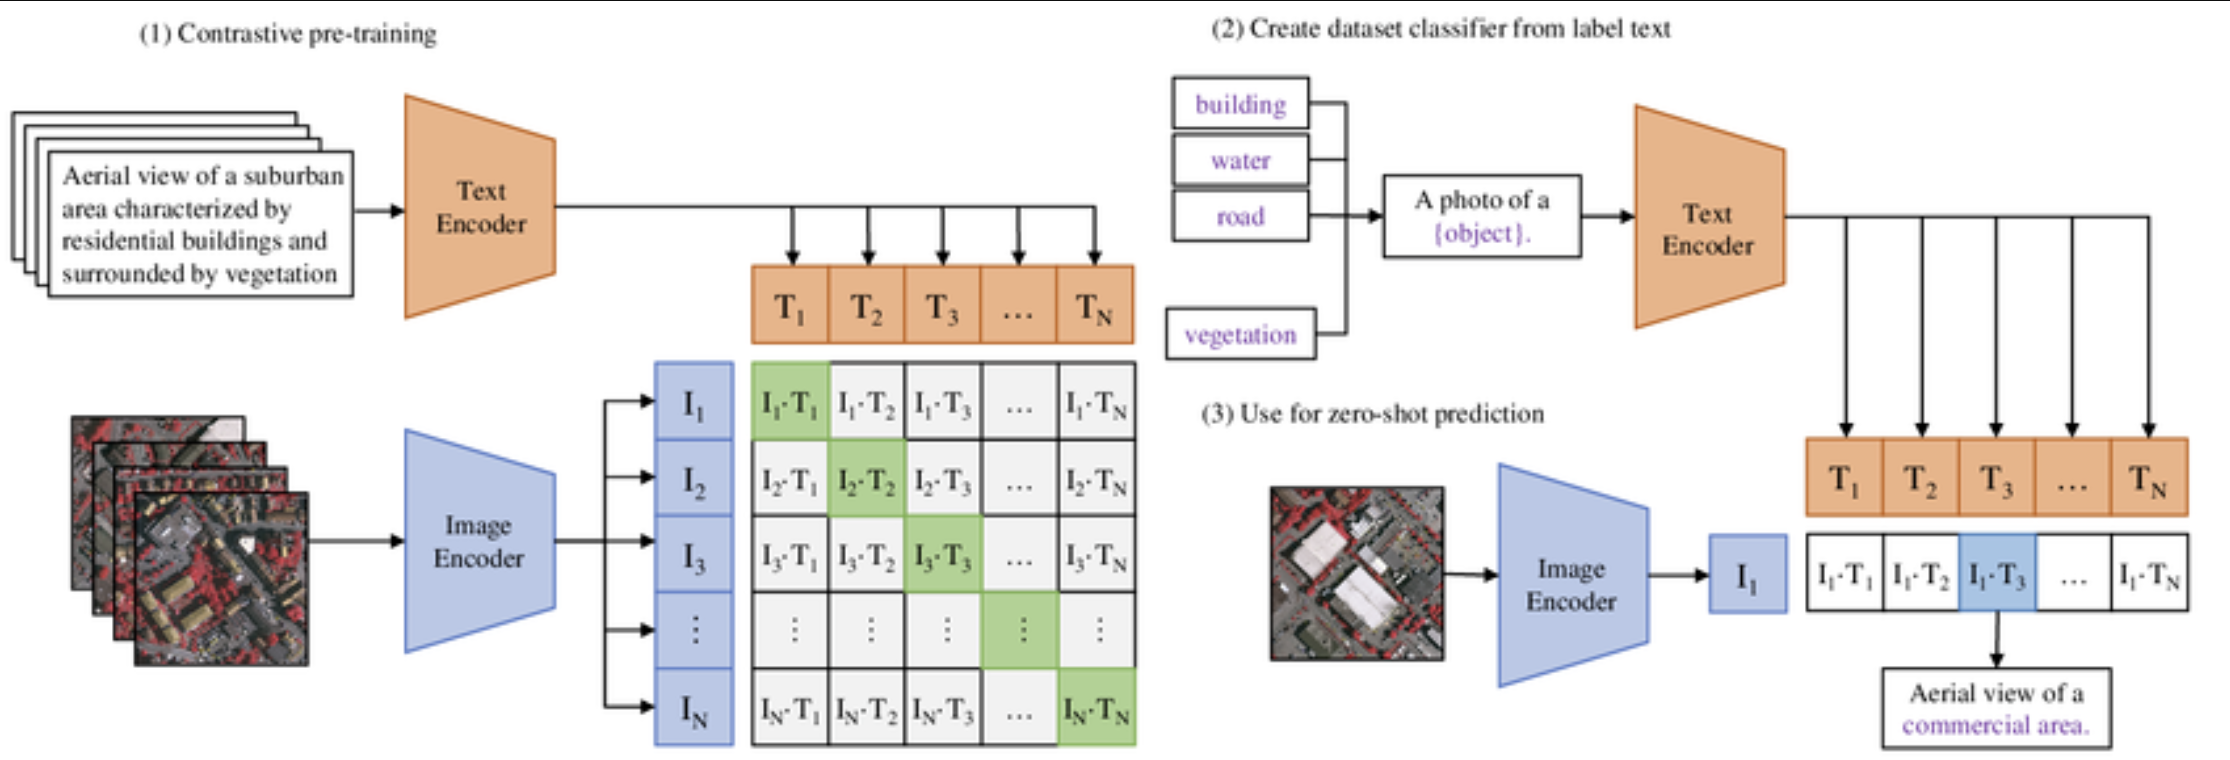
\includegraphics[width=.5\textwidth]{CLIP.png}
            \caption{Arquitetura CLIP}
            \label{fig:CLIP}
	    \end{figure}
        
		\item \textbf{Sistemas de Recomendação de Próxima Geração}: Os modelos clássicos de recomendação baseados em filtragem colaborativa ou matrizes de esparsidade sofrem com o problema de \textit{cold start} e escalabilidade. Os sistemas modernos contornam isso mapeando de forma contínua o comportamento, preferências e histórico do usuário, bem como os atributos textuais e visuais dos itens (produtos, músicas, artigos), em vetores densos contínuos. Ao alinhar os vetores de perfil do usuário e os vetores de catálogo no mesmo espaço geométrico, a recomendação deixa de ser um cruzamento massivo de tabelas relacionais e passa a ser um problema de vizinhança topológica \cite{covington2016deep}. O banco vetorial computa e atualiza essas relações em milissegundos por proximidade geométrica. Isso garante que, mesmo diante de catálogos dinâmicos com milhões de itens, o sistema consiga entregar recomendações personalizadas com latência ultra-baixa no momento em que o usuário interage com a plataforma.

        \begin{figure}[ht]
            \centering
            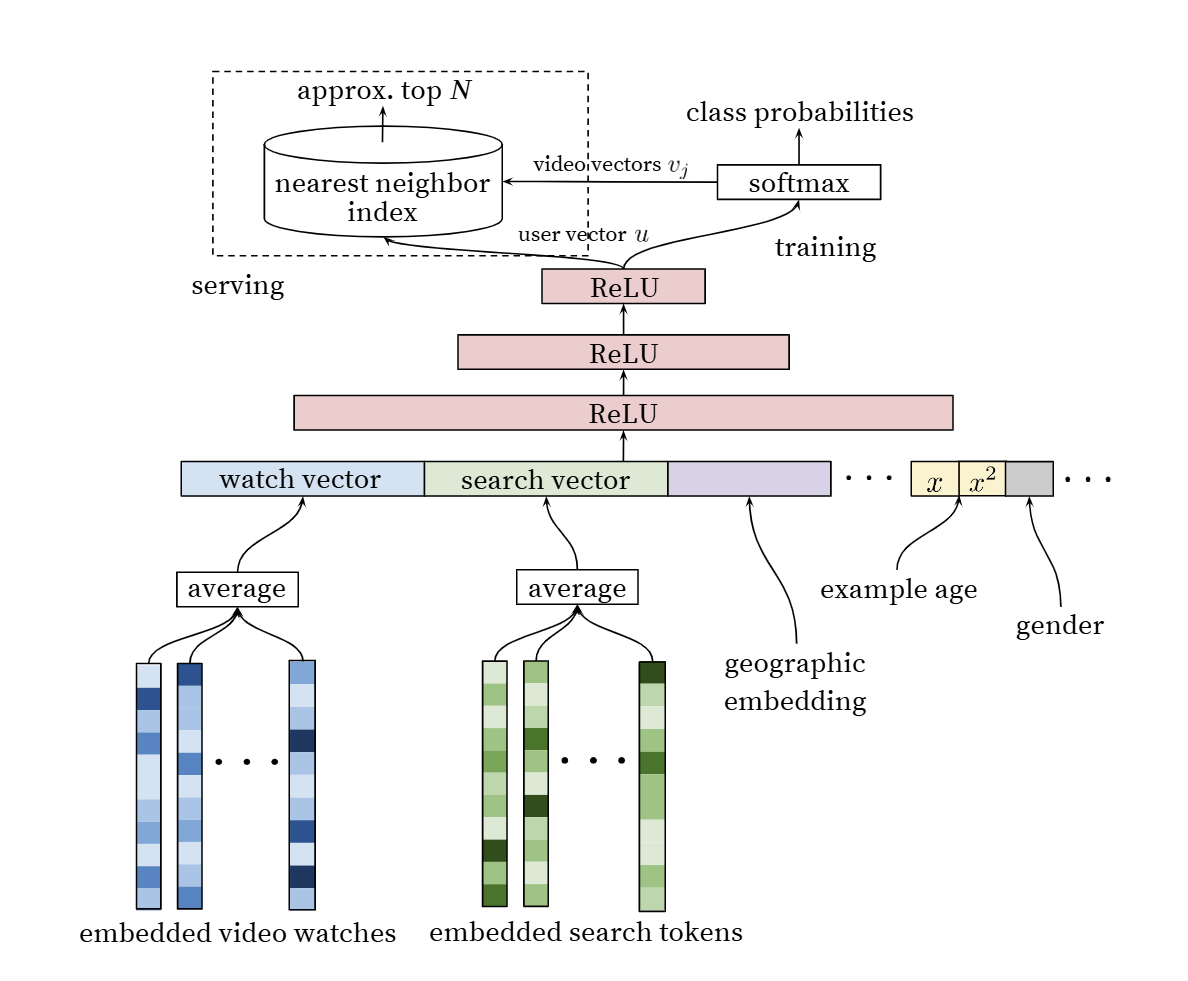
\includegraphics[width=.5\textwidth]{geracao-candidatos.png}
            \caption{Geração de Candidatos}
            \label{fig:Candidatos}
	    \end{figure}
        
	\end{itemize}
	
	\section{Fundamentos Matemáticos das Bases Vetoriais} \label{sec:fundamentos}
    
    \subsection{Transformers}

    O modelo adota uma estrutura clássica de Codificador-Decodificador (Encoder-Decoder).
    
    \subsubsection{Produto escalar de Self-Attention}
    
    A função de atenção mapeia um conjunto de vetores de consulta (Query - $Q$), chaves (Key - $K$) e valores (Value - $V$) num vetor de saída.
    
    A fórmula matemática para computar a atenção sobre matrizes de consultas $Q$, chaves $K$ e valores $V$ é:
    
    $$\text{Attention}(Q, K, V) = \text{softmax}\left(\frac{QK^T}{\sqrt{d_k}}\right)V$$
    
    $Q, K, V$: São matrizes que contêm as representações vetoriais das palavras. No caso da Self-Attention, estas matrizes vêm todas da mesma sequência de entrada original, mas são multiplicadas por matrizes de pesos lineares diferentes.
    
    $QK^T$ (Produto Escalar): Multiplica as consultas pelas chaves transpostas. Isto calcula a afinidade ou similaridade entre cada palavra e todas as outras palavras da frase. Se duas palavras forem semanticamente muito relacionadas naquele contexto, o produto escalar será alto.
    
    $\frac{1}{\sqrt{d_k}}$ (Fator de Escala): Aqui, $d_k$ é a dimensão dos vetores de chave. Para valores grandes de $d_k$, o produto escalar cresce muito em magnitude, empurrando a função softmax para regiões com gradientes extremamente pequenos (o que causa o problema do gradiente que desaparece). Dividir por $\sqrt{d_k}$ estabiliza as magnitudes.
    
    $\text{softmax}$: Transforma as pontuações de afinidade em probabilidades (valores entre 0 e 1 que somam 1). Isto determina quanta atenção cada palavra deve prestar às outras.
    
    Multiplicação por $V$: Finalmente, pondera-se a matriz de Valores pelas probabilidades obtidas no softmax. Palavras com maior peso de atenção contribuirão mais para a representação final da palavra atual.
    
    \subsubsection{Self-Attention de Múltiplas Cabeças}
    
    Em vez de calcular a atenção apenas uma vez com as dimensões completas é mais vantajoso projetar linearmente as matrizes $Q, K, V$ $h$ vezes em subespaços de dimensões menores ($d_k, d_k, d_v$). Isto permite ao modelo focar simultaneamente em diferentes tipos de informação em posições diferentes.
    
    As fórmulas são:
    
    $$\text{MultiHead}(Q, K, V) = \text{Concat}(\text{head}_1, \dots, \text{head}_h)W^O$$
    
    Onde cada cabeça ($\text{head}_i$) é calculada como:
    
    $$\text{head}_i = \text{Attention}(QW_i^Q, KW_i^K, VW_i^V)$$
    
    $W_i^Q \in \mathbb{R}^{d_{model} \times d_k}$, $W_i^K \in \mathbb{R}^{d_{model} \times d_k}$, $W_i^V \in \mathbb{R}^{d_{model} \times d_v}$: São matrizes de projeção linear (pesos que o modelo aprende durante o treino) para a cabeça $i$.
    
    $W^O \in \mathbb{R}^{h \cdot d_v \times d_{model}}$: Uma matriz de pesos finais pela qual o resultado concatenado de todas as cabeças é multiplicado para retornar à dimensão original do modelo ($d_{model} = 512$).
   
    \subsubsection{Feed-Forward Networks (FFN)}
    
    Além das camadas de atenção, cada camada do codificador e do descodificador contém uma rede totalmente conectada (Feed-Forward) que é aplicada a cada palavra de forma independente e idêntica. Ela consiste em duas transformações lineares com uma ativação ReLU no meio:
    
    $$\text{FFN}(x) = \max(0, xW_1 + b_1)W_2 + b_2$$
   
    $x$: O vetor da palavra na posição atual após passar pela camada de atenção.
    
    $\max(0, \cdot)$: Esta é a função de ativação ReLU (Rectified Linear Unit), que introduz não-linearidade no modelo. Se o valor for negativo, torna-se 0; se for positivo, mantém-se igual.
    
    $W_1, b_1, W_2, b_2$: São os pesos e bias das duas camadas lineares. A dimensão interna da FFN é $d_{ff} = 2048$, enquanto a de entrada/saída é $d_{model} = 512$.
  
    \subsubsection{Codificação Posicional}
    
    Como o Transformer não utiliza recorrência (RNNs) nem convoluções (CNNs), ele não sabe a ordem das palavras numa frase. Para resolver isto, o modelo adiciona uma Codificação Posicional aos embeddings:
    
    $$PE_{(pos, 2i)} = \sin\left(\frac{pos}{10000^{\frac{2i}{d_{model}}}}\right)$$
    
    $$PE_{(pos, 2i+1)} = \cos\left(\frac{pos}{10000^{\frac{2i}{d_{model}}}}\right)$$
  
     $pos$: É a posição física da palavra na frase.
     
     $i$: É o índice da dimensão dentro do vetor (varia de $0$ até $d_{model}/2$). As dimensões pares ($2i$) usam a função seno, e as ímpares ($2i+1$) usam a função cosseno.
 
    \subsubsection{Considerações do Bloco Encoder-Decoder}
    
    Cada subcamada (tanto Atenção como FFN) em cada bloco do Transformer emprega uma Conexão Residual seguida por uma Normalização de Camada (Layer Normalization):
    
    $$\text{Saída} = \text{LayerNorm}(x + \text{Sublayer}(x))$$
    
    Isto ajuda no fluxo de gradientes durante a backpropagation, permitindo treinar redes muito profundas sem que os gradientes desapareçam ou explodam.

    
	\subsection{Embeddings}
	
	Seja $\mathcal{D}$ um espaço amostral de dados não estruturados (e.g., um corpus de texto textualmente infinito ou um conjunto discreto de tokens). Um modelo de embedding é definido como um operador de mapeamento não linear parametrizado $\phi: \mathcal{D} \to \mathcal{H}_d$, onde $\mathcal{H}_d \subseteq \mathbb{R}^d$ denota um espaço de Hilbert real de alta dimensionalidade $d \in \mathbb{N}^+$.
    
    Para cada elemento $x \in \mathcal{D}$, o operador $\phi$ injeta as propriedades semânticas latentes de $x$ em um vetor coluna denso $\mathbf{v}$:
    
    $$\mathbf{v} = \phi(x; \Theta) = [v_1, v_2, \dots, v_d]^T \in \mathcal{H}_d$$
    
    onde $\Theta$ representa o tensor de parâmetros (pesos sinápticos) aprendidos pelo modelo durante a otimização de uma função de perda global $\mathcal{L}$.
    
    Em arquiteturas do estado da arte baseadas em Transformers ($d = 768$) ou LLMs comerciais ($d = 1536$ ou $d = 3072$), a dimensão $d$ define o grau de liberdade do espaço latente. Cada componente $v_i$ (para $i = 1, \dots, d$) representa a projeção escalar de $\mathbf{v}$ sobre um vetor ortonormal de uma base canônica $\mathcal{B} = \{\mathbf{e}_1, \mathbf{e}_2, \dots, \mathbf{e}_d\}$ que gera $\mathcal{H}_d$. Esses eixos coordenados correspondem a direções ortogonais em uma variedade latente abstrata, capturando distribuições de características sintáticas, semânticas e contextuais.
    
    O espaço $\mathcal{H}_d$ é necessariamente dotado de uma estrutura métrica interna induzida por um produto escalar $\langle \cdot, \cdot \rangle$, tipicamente avaliada via Similaridade de Cosseno, definida formalmente como:
    
    $$\text{Sim}(\mathbf{v}_i, \mathbf{v}_j) = \frac{\langle \mathbf{v}_i, \mathbf{v}_j \rangle}{\|\mathbf{v}_i\|_2 \|\mathbf{v}_j\|_2} = \frac{\sum_{k=1}^d v_{ik} v_{jk}}{\sqrt{\sum_{k=1}^d v_{ik}^2} \sqrt{\sum_{k=1}^d v_{jk}^2}}$$

    Um Espaço de Hilbert é um espaço vetorial que possui geometria completa. Para que um espaço receba esse título, ele precisa cumprir três requisitos matemáticos rigorosos:

    \begin{itemize}
        \item Possuir um Produto Interno (Produto Escalar): Diferente de um espaço vetorial comum onde você só pode somar e multiplicar vetores por números, no espaço de Hilbert você pode multiplicar dois vetores entre si através de um operador $\langle \mathbf{u}, \mathbf{v} \rangle$.
        \item Induzir Métrica e Norma: A existência do produto interno permite definir o comprimento de um vetor (Norma: $\|\mathbf{u}\| = \sqrt{\langle \mathbf{u}, \mathbf{u} \rangle}$) e a distância entre dois vetores ($d(\mathbf{u}, \mathbf{v}) = \|\mathbf{u} - \mathbf{v}\|$).
        \item Ser Completo (Espaço de Banach): Significa que qualquer sequência de vetores que pareça estar convergindo para algum lugar (sequências de Cauchy) realmente converge para um vetor que também está dentro desse mesmo espaço.
    \end{itemize}
    
    O espaço de embeddings possui um produto interno bem definido, podemos calcular o ângulo entre dois vetores semânticos. Isso permite usar a Similaridade de Cosseno para dizer se a palavra está geometricamente próxima.

    Em alta dimensionalidade, escolher dois vetores totalmente aleatórios no espaço de Hilbert, o ângulo entre eles será quase sempre de 90° (ortogonais). Geometricamente, os vetores tendem a se isolar nos cantos e superfícies do espaço.Para que dois vetores em $d=1536$ tenham uma similaridade de cosseno alta (próxima de 1), a rede neural precisa alinhar de forma extremamente precisa centenas de coordenadas textuais, garantindo que apenas conceitos verdadeiramente correlacionados compartilhem a mesma vizinhança geométrica.
	
	\subsection{Métricas de Distância e Similaridade Vetorial}
	
	A busca semântica em bancos de dados vetoriais consiste em encontrar os vetores logicamente mais próximos de um vetor de query $\mathbf{q} \in \mathbb{R}^d$. Para mensurar essa proximidade, utilizam-se funções que mapeiam o par de vetores para um escalar real. Sejam $\mathbf{u}, \mathbf{v} \in \mathbb{R}^d$:
	
	\subsubsection{Distância Euclidiana ($L_2$)}
	
	Mede a distância geométrica em linha reta entre os pontos finais de dois vetores no espaço euclidiano. É formalmente definida pela norma $L_2$ do vetor diferença:
	
	$$D_{Euclidiana}(\mathbf{u}, \mathbf{v}) = \|\mathbf{u} - \mathbf{v}\|_2 = \sqrt{\sum_{i=1}^{d} (u_i - v_i)^2}$$
	
	Satisfaz todas as condições de uma métrica rígida (não-negatividade, identidade dos indiscerníveis, simetria e a desigualdade triangular: $\|\mathbf{u} - \mathbf{w}\|_2 \le \|\mathbf{u} - \mathbf{v}\|_2 + \|\mathbf{v} - \mathbf{w}\|_2$).
	
	\subsubsection{Similaridade de Cosseno}
	
	Mede o cosseno do ângulo formado entre os dois vetores, focando estritamente na sua orientação e ignorando as suas magnitudes absolutas. É expressa pela razão entre o produto interno e o produto de suas normas:
	
	$$S_{Cosseno}(\mathbf{u}, \mathbf{v}) = \cos(\theta) = \frac{\mathbf{u} \cdot \mathbf{v}}{\|\mathbf{u}\|_2 \|\mathbf{v}\|_2} = \frac{\sum_{i=1}^{d} u_i v_i}{\sqrt{\sum_{i=1}^{d} u_i^2} \sqrt{\sum_{i=1}^{d} v_i^2}}$$
	
	Fornece valores estritamente limitados no intervalo $[-1, 1]$. Em muitos contextos práticos de banco de dados, utiliza-se a \textbf{Distância de Cosseno}, dada por:
    
    $D_{Cosseno}(\mathbf{u}, \mathbf{v}) = 1 - S_{Cosseno}(\mathbf{u}, \mathbf{v})$
	
	\subsubsection{Produto Interno}
	
	Calcula a projeção de um vetor sobre o outro multiplicada por sua magnitude. É comumente utilizado quando os vetores gerados pelo modelo já estão previamente normalizados para possuírem norma unitária ($\|\mathbf{u}\|_2 = \|\mathbf{v}\|_2 = 1$):
	
	$$\text{IP}(\mathbf{u}, \mathbf{v}) = \mathbf{u} \cdot \mathbf{v} = \sum_{i=1}^{d} u_i v_i$$
	
	Se os vetores estão na esfera unitária, o Produto Interno é matematicamente equivalente à Similaridade de Cosseno, reduzindo drasticamente o custo computacional por eliminar o cálculo das raízes quadradas das normas no denominador.

    \subsection{Maldição da Dimensionalidade}

    A tentativa de estender as estruturas de particionamento espacial para o domínio multidimensional por meio de árvores como as $K\text{-d}\text{-Trees}$ ou $\text{R-Trees}$ falha categoricamente devido ao fenômeno matemático conhecido como a maldição da dimensionalidade\cite{bellman1961adaptive}.

    Nas estruturas tipo $K\text{-d}\text{-Trees}$, o espaço é particionado de maneira cíclica ao longo das coordenadas cartesianas através de hiperplanos ortogonais. À medida que o número de dimensões ($d$) cresce, o número de regiões (hipercubos) necessárias para cobrir o espaço amostral cresce exponencialmente à taxa de $2^d$ \cite{weber1998quantitative}. Consequentemente, para um vetor de busca em alta dimensão (onde $d$ frequentemente excede 512 ou 1024), quase todos os caminhos e subárvores da estrutura precisam ser inspecionados durante uma consulta de vizinhos mais próximos ($k\text{-NN}$).

    Considere um hipercubo $d$-dimensional de aresta de comprimento $1$. Seu volume total é dado por $V_{cubo} = 1^d = 1$. Se definirmos uma esfera inscrita nesse cubo com raio $r = 0.5$, o volume dessa hiperesfera é definido por:
	
	$$V_{esfera}(d) = \frac{\pi^{\frac{d}{2}}}{\Gamma\left(\frac{d}{2} + 1\right)} r^d$$
	
	Onde $\Gamma$ representa a função Gamma. Conforme $d \rightarrow \infty$:
	
	$$\lim_{d \rightarrow \infty} V_{esfera}(d) = 0$$
	
	Esse resultado demonstra analiticamente que, em altas dimensões, o volume de uma hiperesfera inscrita torna-se insignificante em relação ao volume do hipercubo que a encerra. Geometricamente, isso implica que quase todo o volume de um hipercubo se concentra nos seus vértices.
    
	Como consequência direta para bancos de dados, os pontos de dados distribuídos aleatoriamente em um espaço de alta dimensão tornam-se equidistantes uns dos outros. A distância máxima e a distância mínima entre quaisquer pares de vetores convergem para o mesmo valor:
	
	$$\lim_{d \rightarrow \infty} \frac{D_{max} - D_{min}}{D_{min}} = 0$$

    \begin{figure}[ht]
        \centering
        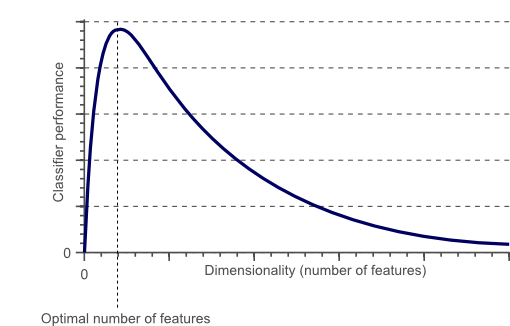
\includegraphics[width=.5\textwidth]{dimensionality_vs_performance.png}
        \caption{Maldição da Dimensionalidade}
        \label{fig:Maldicao}
    \end{figure}
    
    Onde $D_{\max}$ e $D_{\min}$ representam as distâncias máxima e mínima de um ponto de consulta para os pontos do banco de dados, respectivamente. Como a distância entre os vetores se torna homogeneamente uniforme, o conceito de proximidade perde o sentido estatístico. Para o algoritmo de busca na árvore, isso significa que o mecanismo de poda de ramificações se torna ineficaz: o algoritmo é incapaz de descartar subárvores com base em bounding boxes, pois a esfera de busca da consulta inevitavelmente intercepta quase todos os hipercubos do índice.
    
    Como consequência direta dessa degradação estrutural, o comportamento assintótico de busca dessas árvores multidimensionais degenera de $O(\log N)$ para $O(N)$, onde $N$ é o número total de vetores. O SGBD é, portanto, forçado a retroceder para uma varredura sequencial linear (linear scan), calculando exaustivamente a distância (seja Euclidiana, Cosseno ou Produto Interno) entre o vetor de consulta e todos os bilhões de vetores da base de dados. É por este exato motivo que os sistemas de bancos de dados vetoriais abrem mão da exatidão absoluta e adotam algoritmos de Vizinhos Mais Próximos Aproximados (ANN), trocando uma fração infinitesimal de precisão por ganhos de ordens de magnitude em latência e vazão.
	
	\section{Objetivos do Estudo Realizado} \label{sec:objetivos}
		
	
	\section{Métodos Empregados na Condução do Estudo} \label{sec:metodos}
	
	
	
	\section{Principais conceitos relacionados ao tema escolhido} \label{sec:conceitos}
	

	
	\section{Descrição do estudo realizado e apresentação dos seus resultados} \label{sec:caso}
	
	
	
	\section{Discussão sobre os resultados do estudo} \label{sec:resultados}

	
	\bibliographystyle{sbc}
	\bibliography{sbc-template}
	
\end{document}
